\chapter{Instance-level object detection}


\begin{description}
    \item[Instance-level object detection] \marginnote{Instance-level object detection}
        Given a reference/model image of a specific object,
        determine if the object is present in the target image and estimate its pose.

        \begin{remark}
            This is different from category-level object detection which deals with detecting classes of objects
            independent of appearance and pose.
        \end{remark}
\end{description}



\section{Template matching}
\marginnote{Template matching}

Slide the model image (template) across the target image and 
use a similarity/dissimilarity function with a threshold to determine if a match has been found.


\subsection{Similarity/dissimilarity functions}

Let $I$ be the target image and $T$ the template image of shape $M \times N$.
Possible similarity/dissimilarity functions are:
\begin{descriptionlist}
    \item[Pixel-wise intensity differences] \marginnote{Pixel-wise intensity differences}
        Squared difference between the intensities of the template image and the patch in the target image:
        \[ \texttt{SSD}(i, j) = \sum_{m=0}^{M-1} \sum_{n=0}^{N-1} \big( I(i+m, j+n) - T(m, n) \big)^2 \]
        
        \begin{remark}
            \texttt{SSD} is fast but not intensity invariant.
        \end{remark}

    \item[Sum of absolute differences] \marginnote{Sum of absolute differences}
        Difference in absolute value between the intensities of the template image and the patch in the target image:
        \[ \texttt{SAD}(i, j) = \sum_{m=0}^{M-1} \sum_{n=0}^{N-1} \big\vert I(i+m, j+n) - T(m, n) \big\vert \]
        
        \begin{remark}
            \texttt{SAD} is fast but not intensity invariant.
        \end{remark}

    \item[Normalized cross-correlation] \marginnote{Normalized cross-correlation}
        Cosine similarity between the template image and the target image patch (which are seen as flattened vectors):
        \[ 
            \texttt{NCC}(i, j) = 
            \frac{ \sum\limits_{m=0}\limits^{M-1} \sum\limits_{n=0}\limits^{N-1} \big( I(i+m, j+n) \cdot T(m, n) \big) }
                { \sqrt{\sum\limits_{m=0}\limits^{M-1} \sum\limits_{n=0}\limits^{N-1} I(i+m, j+n)^2} \cdot \sqrt{\sum\limits_{m=0}\limits^{M-1} \sum\limits_{n=0}\limits^{N-1} T(m, n)^2} } 
        \]

        In other words, let $\tilde{I}_{i,j}$ be a $M \times N$ patch of the target image $I$ starting at the coordinates $(i, j)$.
        In vector form, $\texttt{NCC}(i, j)$ computes the cosine of the angle $\theta$ between $\tilde{I}_{i,j}$ and $T$.
        \[ \texttt{NCC}(i, j) = \frac{\tilde{I}_{i,j} \cdot T}{\Vert \tilde{I}_{i,j} \Vert \cdot \Vert T \Vert} = \cos \theta \]

        \begin{remark}
            \texttt{NCC} is invariant to a linear intensity change but not to an additive bias.
        \end{remark}

    \item[Zero-mean normalized cross-correlation] \marginnote{Zero-mean normalized cross-correlation}
        Let $\tilde{I}_{i,j}$ be a $M \times N$ patch of $I$ starting at the coordinates $(i, j)$.
        Zero-mean normalized cross-correlation subtracts the mean of the template image and the patch of the target image
        before computing \texttt{NCC}:
        \[ \mu(\tilde{I}_{i,j}) = \frac{1}{MN} \sum_{m=0}^{M-1} \sum_{n=0}^{N-1} I(i+m, j+n) \hspace{3em} \mu(T) = \frac{1}{MN} \sum_{m=0}^{M-1} \sum_{n=0}^{N-1} T(m, n) \]
        \[ 
            \texttt{ZNCC}(i, j) = 
            \frac{ \sum\limits_{m=0}\limits^{M-1} \sum\limits_{n=0}\limits^{N-1} \Big( \big(I(i+m, j+n) - \mu(\tilde{I}_{i,j})\big) \cdot \big(T(m, n) - \mu(T)\big) \Big) }
                { \sqrt{\sum\limits_{m=0}\limits^{M-1} \sum\limits_{n=0}\limits^{N-1} \big(I(i+m, j+n) - \mu(\tilde{I}_{i,j})\big)^2} \cdot \sqrt{\sum\limits_{m=0}\limits^{M-1} \sum\limits_{n=0}\limits^{N-1} \big(T(m, n) - \mu(T)\big)^2} } 
        \]

        \begin{remark}
            \texttt{ZNCC} is invariant to an affine intensity change.
        \end{remark}
\end{descriptionlist}

\begin{figure}[H]
    \centering
    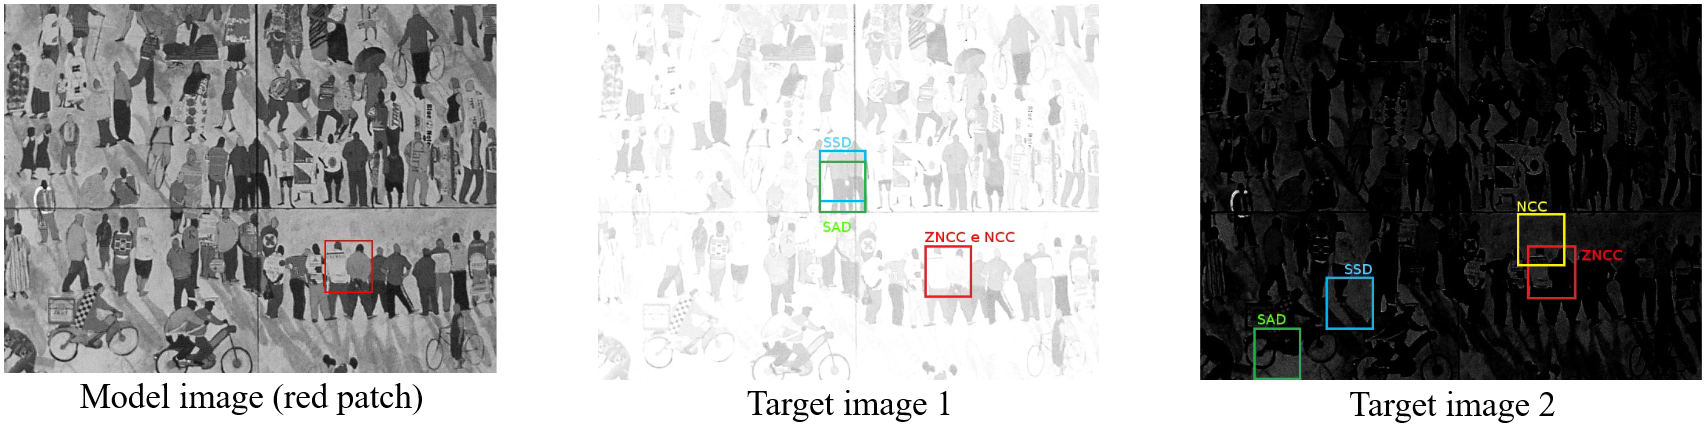
\includegraphics[width=0.95\linewidth]{./img/template_matching_example.png}
    \caption{Examples of template matching}
\end{figure}



\section{Shape-based matching}
\marginnote{Shape-based matching}

Edge-based template matching that works as follows:
\begin{enumerate}
    \item Use an edge detector to extract a set of control points $\{ P_1, \dots, P_n \}$ in the template image $T$.
    \item Compute the gradient normalized to unit vector at each point $P_k$:
        \[ \nabla T(P_k) = \begin{pmatrix} \partial_x T(P_k) \\ \partial_y T(P_k) \end{pmatrix} \hspace{2em} \vec{u}_k(P_k) = \frac{\nabla T(P_k)}{\Vert \nabla T(P_k) \Vert} \]
    \item Given a patch $\tilde{I}_{i,j}$ of the target image, 
        compute the gradient normalized to unit vector at the points $\{ \tilde{P}_1(i, y), \dots, \tilde{P}_n(i, y) \}$ 
        corresponding to the control points of the template image:
        \[ 
            \nabla \tilde{I}_{i,j}(\tilde{P}_k) = \begin{pmatrix} \partial_x \tilde{I}_{i,j}(\tilde{P}_k) \\ \partial_y \tilde{I}_{i,j}(\tilde{P}_k) \end{pmatrix} \hspace{2em} 
            \tilde{\vec{u}}_k(\tilde{P}_k) = \frac{\nabla \tilde{I}_{i,j}(\tilde{P}_k)}{\Vert \nabla \tilde{I}_{i,j}(\tilde{P}_k) \Vert} 
        \]
    \item Compute the similarity as the mean of the cosine similarities of each pair of gradients:
        \[ S(i, j) = \frac{1}{n} \sum_{k=1}^{n} \vec{u}_k(P_k) \cdot \tilde{\vec{u}}_k(\tilde{P}_k) = \frac{1}{n} \sum_{k=1}^{n} \cos \theta_k \in [-1, 1] \]
        $S(i, j) = 1$ when the gradients perfectly match. A minimum threshold $S_\text{min}$ is used to determine if there is a match.
\end{enumerate}

\begin{figure}[H]
    \centering
    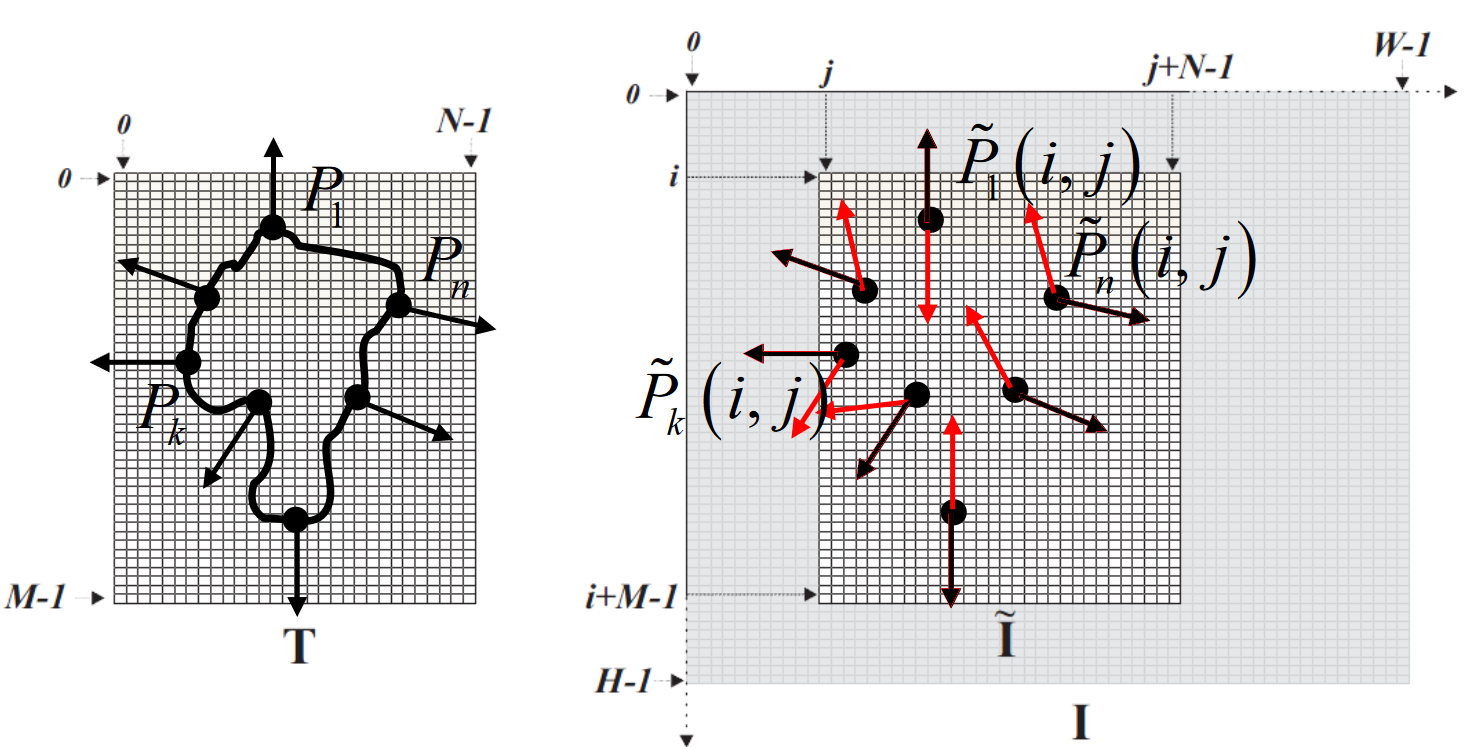
\includegraphics[width=0.5\linewidth]{./img/shape_based_matching.png}
    \caption{Example of control points matching}
\end{figure}


\subsection{Invariance to global inversion of contrast polarity}

As an object might appear on a darker or brighter background, more robust similarity functions can be employed:
\begin{description}
    \item[Global polarity inversion contrast] 
        \[ S(i, j) = \frac{1}{n} \left\vert \sum_{k=1}^{n} \vec{u}_k(P_k) \cdot \tilde{\vec{u}}_k(\tilde{P}_k) \right\vert = 
            \frac{1}{n} \left\vert \sum_{k=1}^{n} \cos \theta_k \right\vert \]

    \item[Local polarity inversion contrast] 
        \[ S(i, j) = \frac{1}{n} \sum_{k=1}^{n} \left\vert  \vec{u}_k(P_k) \cdot \tilde{\vec{u}}_k(\tilde{P}_k) \right\vert = 
        \frac{1}{n} \sum_{k=1}^{n} \left\vert \cos \theta_k \right\vert \]

        \begin{remark}
            This is the most robust one.
        \end{remark}
\end{description}



\section{Hough transform}

Detect objects of a known shape that can be expressed through an analytic equation 
by means of a projection from the image space to a parameter space.

\begin{description}
    \item[Parameter space] \marginnote{Parameter space}
        Euclidean space parametrized on the parameters $\phi$ of an analytic shape $\mathcal{S}_\phi$ (e.g. line, sphere, \dots).
        A point $(x, y)$ in the image space is projected into the curve (which also intends lines) that contains the set of parameters $\hat{\phi}$
        such that the shape $\mathcal{S}_{\hat{\phi}}$ defined on those parameters passes through $(x, y)$ in the image space.

        \begin{remark}
            If many curves intersect at $\hat{\phi}$ in the parameter space of a shape $S_\phi$, then, there is high evidence of the fact that 
            the image points that were projected into those curves are part of the shape $S_{\hat{\phi}}$.
        \end{remark}

        \begin{example}[Space of straight lines] 
            Consider the line equation:
            \[ \hat{y} - m\hat{x} - c = 0 \]
            where $(\hat{x}, \hat{y})$ are fixed while $(m, c)$ vary (in the usual equation, it is the opposite).

            This can be seen as a mapping of points $(\hat{x}, \hat{y})$ into the space
            of points $(m, c)$ such that the straight line parametrized on $m$ and $c$ passes through $(\hat{x}, \hat{y})$
            (i.e. a point in the image space is mapped into a line in the parameter space as infinite lines pass through a point).

            For instance, consider two points $p_1$, $p_2$ in the image space and
            their projection in the parameter space.
            If the two lines intersect at the point $(\tilde{m}, \tilde{c})$,
            then the line parametrized on $\tilde{m}$ and $\tilde{c}$ passes through both $p_1$ and $p_2$ in the image space.
            
            \begin{figure}[H]
                \centering
                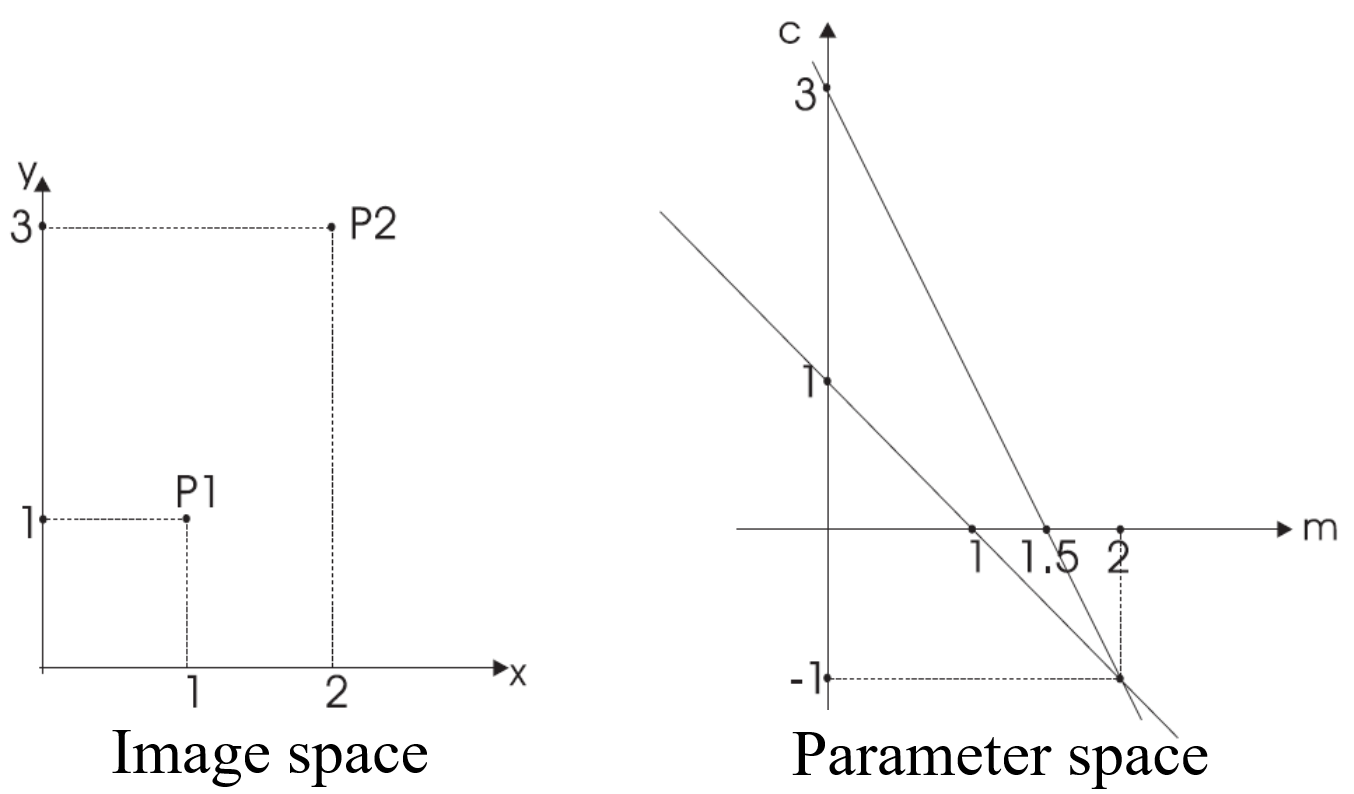
\includegraphics[width=0.4\linewidth]{./img/hough_line_parameter_space.png}
            \end{figure}

            \indenttbox
            \begin{remark}
                By projecting $n$ points of the image space, there are at most $\frac{n(n-1)}{2}$ intersections in the parameter space.
            \end{remark}
        \end{example}

    \item[Algorithm] \marginnote{Object detection using Hough transform}
        Given an analytic shape that we want to detect, 
        object detection using the Hough transform works as follows:
        \begin{enumerate}
            \item Map image points into curves of the parameter space.
            \item The parameter space is quantized into $M \times N$ cells and an accumulator array $A$ of the same shape is initialized to $0$.
            \item For each cell $(i, j)$ of the discretized grid, 
                the corresponding cell $A(i, j)$ in the accumulator array counts how many curves lie in that cell (i.e. voting process).
            \item Find the local maxima of $A$ and apply a threshold if needed.
                The points that were projected into the curves passing through a maximum cell are points belonging to an object of the sought shape.
        \end{enumerate}
        
        \begin{remark}
            The Hough transform reduces a global detection problem into a local detection in the parameter space.
        \end{remark}

        \begin{remark}
            The Hough transform is usually preceded by an edge detection phase so that the input consists of the edge pixels of the image.
        \end{remark}

        \begin{remark}
            The Hough transform is robust to noise and can detect partially occluded images (with a suitable threshold).
        \end{remark}
\end{description}


\subsection{Hough transform for line detection}
\marginnote{Hough transform for line detection}

For line detection, points in the image space are projected into lines of the parameter space.

\begin{figure}[H]
    \centering
    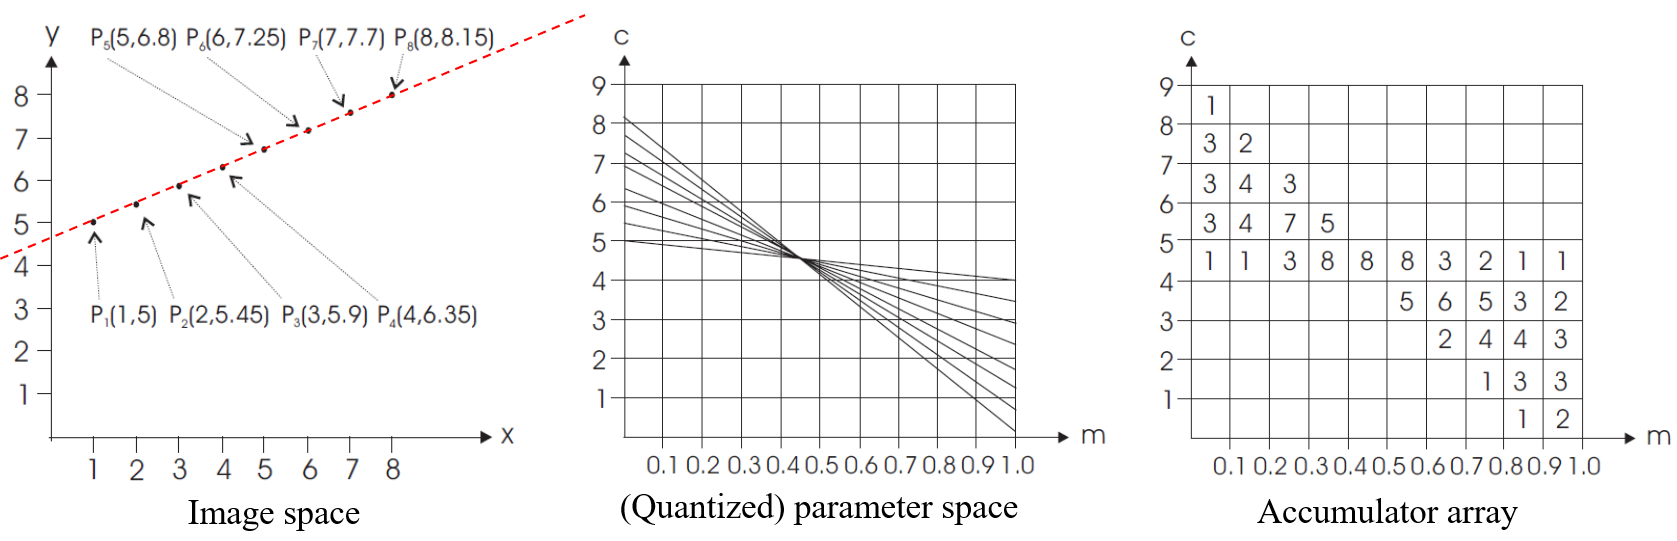
\includegraphics[width=0.85\linewidth]{./img/hough_line_detection.png}
    \caption{Example of line detection}
\end{figure}

In practice, the parametrization on $(m, c)$ of the equation $y-mx-c = 0$ is impractical as $m$ and $c$ have an infinite range.
An alternative approach is to describe straight lines as linear trigonometric equations parametrized on $(\theta, \rho)$:
\[ x \cos \theta + y \sin \theta - \rho = 0 \]
In this form, $\theta \in [ -\frac{\pi}{2}, \frac{\pi}{2} ]$ while $\rho \in [-\rho_\text{max}, \rho_\text{max}]$
where $\rho_\text{max}$ is usually taken of the same size as the diagonal of the image (e.g. for square $N \times N$ images, $\rho_\text{max} = N\sqrt{2}$).



\section{Generalized Hough transform}

Hough transform extended to detect an arbitrary shape.


\subsection{Naive approach}

\begin{description}
    \item[Off-line phase] \marginnote{Generalized Hough transform}
        Phase in which the model of the template object is built.
        Given a template shape, the algorithm works as follows:
        \begin{enumerate}
            \item Fix a reference point $\vec{y}$ (barycenter). $\vec{y}$ is typically within the shape of the object.
            \item For each point $\vec{x}$ at the border $B$ of the object:
                \begin{enumerate}
                    \item Compute its gradient direction $\varphi(\vec{x})$ and discretize it according to a chosen step $\Delta \varphi$.
                    \item Compute the vector $\vec{r} = \vec{y} - \vec{x}$ as the distance of $\vec{x}$ to the barycenter.
                    \item Store $\vec{r}$ as a function of $\Delta \varphi$ in a table (R-table).
                        Note that more than one vector might be associated with the same $\Delta \varphi$.
                \end{enumerate}
        \end{enumerate}
        
        \begin{example}
            \phantom{}\\[0.5em]
            \begin{minipage}{0.7\linewidth}
                \small
                \begin{tabular}{lll}
                    \toprule
                    $i$ & $\varphi_i$ & $R_{\varphi_i}$ \\
                    \midrule
                    $0$ & $0$                   & $\{ \vec{r} \mid \vec{r}=\vec{y}-\vec{x}.\, \forall \vec{x} \in B: \varphi(\vec{x}) = 0 \}$ \\
                    $1$ & $\Delta\varphi$       & $\{ \vec{r} \mid \vec{r}=\vec{y}-\vec{x}.\, \forall \vec{x} \in B: \varphi(\vec{x}) = \Delta\varphi \}$ \\
                    $2$ & $2\Delta\varphi$      & $\{ \vec{r} \mid \vec{r}=\vec{y}-\vec{x}.\, \forall \vec{x} \in B: \varphi(\vec{x}) = 2\Delta\varphi \}$ \\
                    \multicolumn{1}{c}{\vdots} & \multicolumn{1}{c}{\vdots} & \multicolumn{1}{c}{\vdots} \\
                    \bottomrule
                \end{tabular}
            \end{minipage}
            \begin{minipage}{0.2\linewidth}
                \centering
                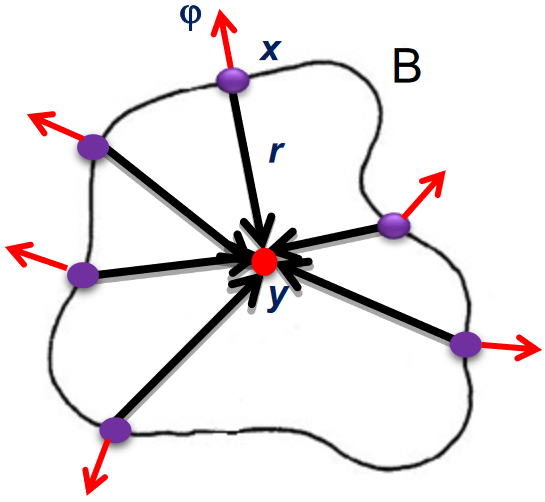
\includegraphics[width=\linewidth]{./img/generalized_hough_offline.png}
            \end{minipage}
        \end{example}

    \item[On-line phase]
        Phase in which the object is detected.
        Given a $M \times N$ image, the algorithm works as follows:
        \begin{enumerate}
            \item Find the edges $E$ of the image.
            \item Initialize an accumulator array $A$ of the same shape of the image.
            \item For each edge pixel $\vec{x} \in E$:
                \begin{enumerate}
                    \item Compute its gradient direction $\varphi(\vec{x})$ discretized to match the step $\Delta \varphi$ of the R-table.
                    \item For each $\vec{r}_i$ in the corresponding row of the R-table:
                    \begin{enumerate}
                        \item Compute an estimate of the barycenter as $\vec{y} = \vec{x} + \vec{r}_i$.
                        \item Cast a vote in the accumulator array $A[\vec{y}] \texttt{+=} 1$
                    \end{enumerate}
                \end{enumerate}
            \item Find the local maxima of the accumulator vector to estimate the barycenters.
                The shape can then be visually found by overlaying the template barycenter to the found barycenters.
        \end{enumerate}
\end{description}

\begin{remark}
    This approach is not rotation and scale invariant.

    Therefore, if rotation or scale is changed, the method should try different rotations or scales.
\end{remark}


\subsection{Star model}
\marginnote{Star model}

Generalized Hough transform based on local invariant features.

% \begin{remark}
%     Local invariant features usually prune features found along edges.
% \end{remark}

\begin{description}
    \item[Off-line phase] 
        Given a template, its model is obtained as follows:
        \begin{enumerate}
            \item Detect local invariant features $F = \{ F_1, \dots, F_N \}$ and compute their descriptors.
                Each feature $F_i$ is described by the tuple:
                \[ F_i = (\vec{P}_i, \varphi_i, S_i, \vec{D}_i) = \text{(position, canonical orientation, scale, descriptor)} \]
            \item Compute the position of the barycenter $\vec{P}_C$ as:
                \[ \vec{P}_C = \frac{1}{N} \sum_{i=1}^{N} \vec{P}_i \]
            \item For each feature $F_i$ compute the joining vector $\vec{V}_i = \vec{P}_C - \vec{P}_i$ as the distance to the barycenter
                and add it to its associated tuple to obtain:
                \[ F_i = (\vec{P}_i, \varphi_i, S_i, \vec{D}_i, \vec{V}_i) \]
        \end{enumerate}

        \begin{figure}[H]
            \centering
            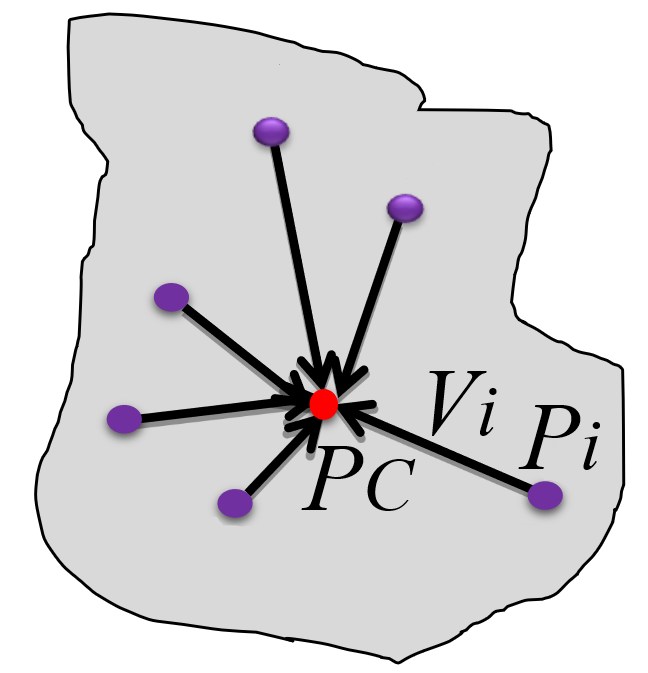
\includegraphics[width=0.2\linewidth]{./img/star_model_offline.png}
        \end{figure}

        \begin{remark}
            The R-table is not needed anymore.
        \end{remark}

    \item[On-line phase] 
        Given a target image, detection works as follows:
        \begin{enumerate}
            \item Extract the local invariant features $\tilde{F} = \{ \tilde{F}_1, \dots, \tilde{F}_M \}$ of the target image.
                Each feature $\tilde{F}_i$ is describe by the tuple:
                \[ \tilde{F}_i = (\tilde{\vec{P}}_i, \tilde{\varphi}_i, \tilde{S}_i, \tilde{\vec{D}}_i) \]
            \item Match the features $\tilde{F}$ of the target image to the features $F$ of the template image through the descriptors.
            \item Initialize a 4-dimensional accumulator array. Two dimensions match the image shape. 
                The other two represent different rotations and scales.
            \item For each target feature $\tilde{F}_i = (\tilde{\vec{P}}_i, \tilde{\varphi}_i, \tilde{S}_i, \tilde{\vec{D}}_i)$ 
                with matching template feature $F_j = (\vec{P}_j, \varphi_j, S_j, \vec{D}_j, \vec{V}_j)$:
                \begin{enumerate}
                    \item Align the joining vector $\vec{V}_j$ to the scale and rotation of $\tilde{F}_i$.
                        
                        Let $\matr{R}(\phi)$ be a $\phi$ degree rotation matrix. The aligned joining vector $\tilde{\vec{V}}_i$ is obtained as:
                        \[ \Delta \varphi_i = \tilde{\varphi}_i - \varphi_j \hspace{3em} \Delta S_i = \frac{\tilde{S}_i}{S_j} \]
                        \[ \tilde{\vec{V}}_i = \Delta S_i \cdot \matr{R}(\Delta \varphi_i) \vec{V}_i \]
                    \item Estimate the barycenter $\tilde{\vec{P}}_{C_i}$ associated to the feature $\tilde{F}_i$ as:
                        \[ \tilde{\vec{P}}_{C_i} = \tilde{\vec{P}}_i + \tilde{\vec{V}}_i \]
                        \begin{figure}[H]
                            \centering
                            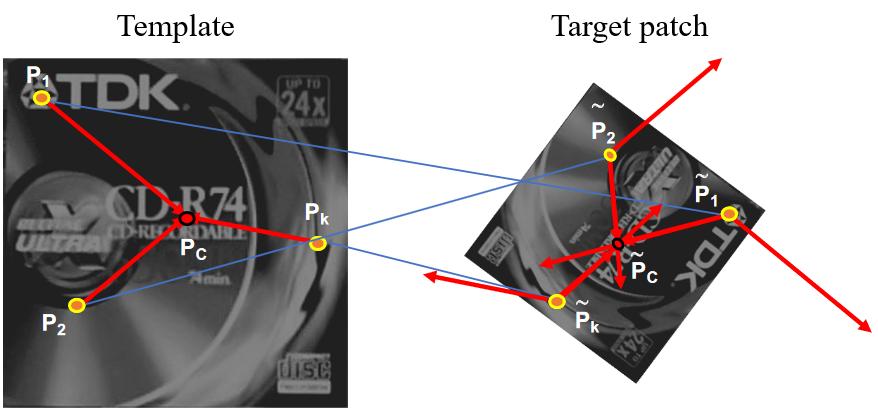
\includegraphics[width=0.55\linewidth]{./img/star_model_online.png}
                        \end{figure}
                    \item Cast a vote in the accumulator array $A[\tilde{\vec{P}}_{C_i}, \Delta S_i, \Delta \varphi_i] \texttt{+=} 1$.
                \end{enumerate}
            \item Find the local maxima of the accumulator vector to estimate the barycenters.
                The shape can then be visually found by overlaying the template barycenter to the found barycenters with the proper scaling and rotation.
                \begin{figure}[H]
                    \centering
                    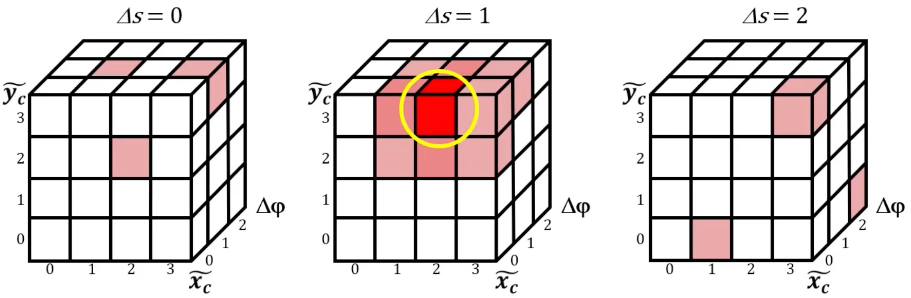
\includegraphics[width=0.6\linewidth]{./img/star_model_voting.png}
                \end{figure}
        \end{enumerate}
\end{description}